\documentclass[aspectratio=169, 10pt]{beamer}

\usepackage{bm} % bold math
\usepackage{fontspec}
\usepackage{minted}
\usepackage{pgf-pie}
\usepackage{tikz}

% Custom commands and environments
\makeatletter
\newcommand\version[1]{\renewcommand\@version{#1}}
\newcommand\@version{}
\def\insertversion{\@version}

\newcommand\course[1]{\renewcommand\@course{#1}}
\newcommand\@course{}
\def\insertcourse{\@course}

\newcommand\coursetitle[1]{\renewcommand\@coursetitle{#1}}
\newcommand\@coursetitle{}
\def\insertcoursetitle{\@coursetitle}

\newcommand\lecturenumber[1]{\renewcommand\@lecturenumber{#1}}
\newcommand\@lecturenumber{}
\def\insertlecturenumber{\@lecturenumber}
\makeatother

\newcommand{\slidetitle}[1]{{\xbseries \large \structure{#1}} \bigskip}
\newcommand{\term}[1]{{\color{blue} #1}}
\newcommand{\leftspace}{\hspace{1em}}
\newcommand{\inlinearrow}{
  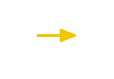
\begin{tikzpicture}[baseline]
    \node [anchor=base] (x) {};
    \draw [rawarrow] (x.mid west) -- ($(x.mid west) + (2em,0)$);
  \end{tikzpicture}
}

\newenvironment{slide}
{\begin{frame}[fragile,environment=slide]\vskip0pt plus 1filll}
{\vskip0pt plus 1filll\end{frame}}

% LaTeX

\setlength{\leftmargini}{1em}

% Common Information

\author{Jon Eyolfson}
\course{ECE 353}
\coursetitle{Systems Software}
\date{2024 Winter}

% fontspec

\defaultfontfeatures{Ligatures=TeX}
% \setmainfont{Domine}
\setsansfont{Inter}[
  FontFace={ul}{n}{Font=*-Thin},
  FontFace={el}{n}{Font=*-ExtraLight},
  FontFace={l}{n}{Font=*-Light},
  FontFace={sb}{n}{Font=*-SemiBold},
  FontFace={eb}{n}{Font=*-ExtraBold},
  FontFace={xb}{n}{Font=*-Black},
]
\setmonofont[Contextuals=AlternateOff, Ligatures=TeXOff]{Iosevka}[
  FontFace={xb}{n}{Font=*-Heavy},
]

%% Font Weights

\DeclareRobustCommand{\ulseries}{\fontseries{ul}\selectfont}
\DeclareTextFontCommand{\textul}{\ulseries}
\DeclareRobustCommand{\elseries}{\fontseries{el}\selectfont}
\DeclareTextFontCommand{\textel}{\elseries}
\DeclareRobustCommand{\lseries}{\fontseries{l}\selectfont}
\DeclareTextFontCommand{\textl}{\lseries}
\DeclareRobustCommand{\sbseries}{\fontseries{sb}\selectfont}
\DeclareTextFontCommand{\textsb}{\sbseries}
\DeclareRobustCommand{\ebseries}{\fontseries{eb}\selectfont}
\DeclareTextFontCommand{\texteb}{\ebseries}
\DeclareRobustCommand{\xbseries}{\fontseries{xb}\selectfont}
\DeclareTextFontCommand{\textxb}{\xbseries}

% tikz

\usetikzlibrary{
  arrows,
  arrows.meta,
  automata,
  backgrounds,
  calc,
  decorations.pathreplacing,
  matrix,
  positioning,
  overlay-beamer-styles,
  shapes,
  shapes.multipart,
  tikzmark,
}

\tikzstyle{rawarrow} = [
  -{Latex[round]},
  line width=1pt,
  yellow,
  shorten >=3pt,
  shorten <=3pt,
  font=\small,
  text=black,
]

\tikzstyle{arrow} = [
  -{Latex[round]},
  line width=1pt,
  yellow,
  shorten >=3pt,
  shorten <=3pt,
  transform canvas={yshift=3pt},
  font=\small,
  text=black,
]

\newcommand{\tikzmarkcoord}[1]{([yshift=3pt]pic cs:#1)}

% minted

\setminted{style=eyolfson, fontsize=\small, escapeinside=||}
\setmintedinline{fontsize=\normalsize}

% hyperref

\hypersetup{colorlinks, urlcolor=blue}

% beamer
\setbeamersize{text margin left=16mm, text margin right=16mm}
\setbeamertemplate{itemize items}[circle]
\setbeamercolor{item}{fg=black}
\setbeamercolor{structure}{fg=darkblue}
\setbeamerfont{frametitle}{series=\bfseries, parent=structure}
\setbeamertemplate{navigation symbols}{}
\setbeamertemplate{headline}{}
\setbeamertemplate{footline}{
  \begin{tikzpicture}[
    remember picture,
    overlay,
    shift={(current page.south west)},
  ]
    \path [fill=gray] (144mm, 0) -- (160mm, 16mm) -- (160mm, 0);
    \node [inner sep=3.5mm, outer sep=0, text=black, anchor=base east,
           align=right, yshift=3.5mm]
          at (current page.south east) {\ttfamily \small \insertframenumber{}};
  \end{tikzpicture}
}
\setbeamertemplate{title page}{
  \begin{tikzpicture}[
    remember picture,
    overlay,
    shift={(current page.south west)},
    background rectangle/.style={fill=darkblue},
    show background rectangle,
  ]
    \node [anchor=center, align=center, text=white, text width=40mm, scale=3.2]
          at (\paperwidth / 2, \paperheight * 2 / 3)
          {\xbseries \inserttitle{}};
    \node [anchor=base west, align=left, inner sep=0, text=white, yshift=2.5mm]
          at (16mm, \paperheight / 3)
          {\insertdate{} \insertcourse{}: \insertcoursetitle{}};
    \node [anchor=base west, align=left, inner sep=0, text=white, yshift=-2.5mm]
          at (16mm, \paperheight / 3)
          {\insertauthor};
    \node [anchor=base east, align=right, inner sep=0, text=white, yshift=2.5mm]
          at (144mm, \paperheight / 3)
          {Lecture \insertlecturenumber{}};
    \node [anchor=base east, align=right, inner sep=0, text=white,
           yshift=-2.5mm]
          at (144mm, \paperheight / 3)
          {\ttfamily \insertversion{}};
    \node [align=center, anchor=south, inner sep=0, text=white, yshift=3.5mm]
          (license) at (\paperwidth / 2, 0)
          {\fontsize{7pt}{7pt}\selectfont This  work is licensed under a
           \href{http://creativecommons.org/licenses/by-sa/4.0/}
                {\color{lightblue} Creative Commons Attribution-ShareAlike 4.0
                 International License}};
  \end{tikzpicture}
}

% xcolor

%% Primary Colour

\definecolor{pantone655}{RGB}{0, 42, 92} % #002a5c
\colorlet{darkblue}{pantone655}

%% Secondary Colours

\definecolor{pantone633}{RGB}{0, 139, 176} % #008bb0
\colorlet{blue}{pantone633}

\definecolor{pantonewarmred}{RGB}{220, 70, 51} % #dc4633
\colorlet{red}{pantonewarmred}

\definecolor{pantone3285}{RGB}{0, 161, 137} % #00a189
\colorlet{cyan}{pantone3285}

\definecolor{pantone7722}{RGB}{13, 83, 77} % #0d534d
\colorlet{darkcyan}{pantone7722}

\definecolor{pantone376}{RGB}{141, 191, 46} % #8dbf2e
\colorlet{green}{pantone376}

\definecolor{pantone2613}{RGB}{109, 36, 122} % #6d247a
\colorlet{violet}{pantone2613}

\definecolor{pantone2985}{RGB}{111, 199, 234} % #6fc7ea
\colorlet{lightblue}{pantone2985}

\definecolor{pantone227}{RGB}{171, 19, 104} % #ab1368
\colorlet{magenta}{pantone227}

\definecolor{pantone7406}{RGB}{241, 197, 0} % #f1c500
\colorlet{yellow}{pantone7406}

%% Neutrals

\definecolor{pantonecoolgray2}{RGB}{208, 209, 201} % #d0d1c9
\colorlet{gray}{pantonecoolgray2}


\lecturenumber{4}
\title{Process Creation}
\version{2.0.0}

\begin{document}
  \begin{frame}[plain, noframenumbering]
    \titlepage
  \end{frame}

  \begin{slide}
    
    \slidetitle{Recall: A Process is an Instance of a Running Program}
  
    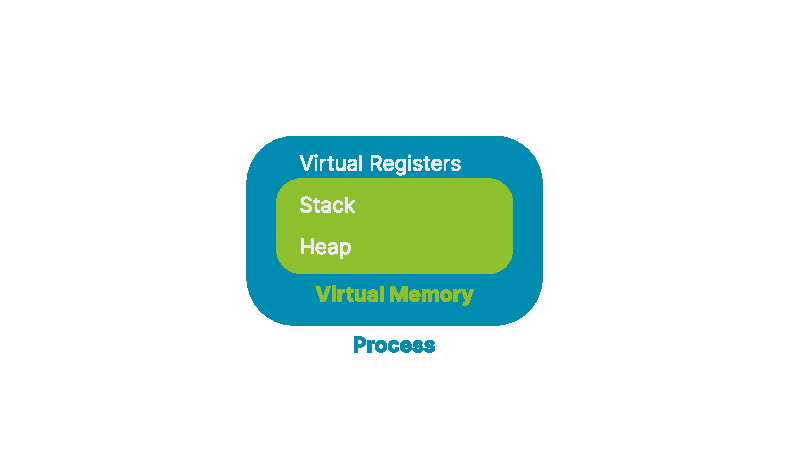
\includegraphics{../01-why-operating-systems/process-virtual-memory.eps}

  \end{slide}

  \begin{slide}

    \slidetitle{We Can Add More to a Process}

    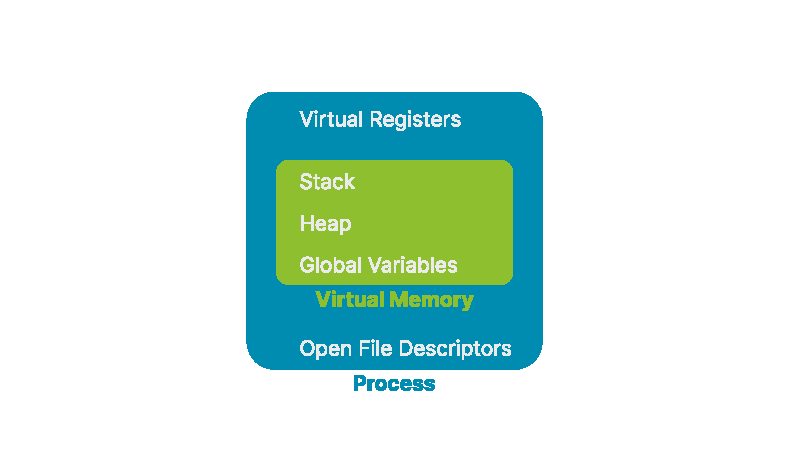
\includegraphics{process.eps}

  \end{slide}

  \begin{slide}
    
    \slidetitle{A Process Control Block (PCB) Contains All Information}

    Specifically, in Linux, this is the \texttt{\color{blue}
    task\_struct} you can browse on

    \href{https://github.com/torvalds/linux/blob/master/include/linux/sched.h\#L743}
         {GitHub}
    \medskip

    It contains:
    \begin{itemize}
      \item Process state
      \item CPU registers
      \item Scheduling information
      \item Memory management information
      \item I/O status information
      \item Any other type of accounting information
    \end{itemize}
    \medskip

    Each process gets a unique process ID (pid) to keep track of it

  \end{slide}

  \begin{slide}
    \slidetitle{Process State Diagram (You Could Rename Waiting to Ready)}

    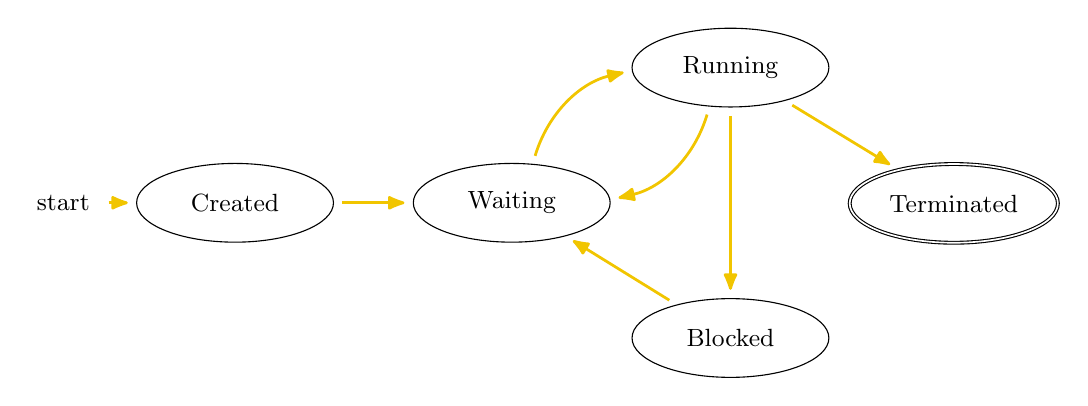
\begin{tikzpicture}[
      every initial by arrow/.style={rawarrow},
      every state/.style={ellipse, minimum width=2.5cm, minimum height=1cm, font=\small},
    ]
      \node [state, initial] (created) {Created};
      \node [state, right=of created] (waiting) {Waiting};
      \node [state, above right=of waiting] (running) {Running};
      \node [state, below right=of waiting] (blocked) {Blocked};
      \node [state, accepting, below right=of running] (terminated) {Terminated};
      \path [rawarrow] (created) edge (waiting)
                 (waiting) edge [bend left] (running)
                 (running) edge [bend left] (waiting)
                 (running) edge (blocked)
                 (blocked) edge (waiting)
                 (running) edge (terminated);
    \end{tikzpicture}
  \end{slide}

  \begin{slide}
    
    \slidetitle{You Can Read Process State Using the ``proc''
                Filesystem}

    There's a standard \texttt{/proc} directory (on Linux) that represents the kernel's
    state

    \leftspace{}These aren't real files, they just look like it!
    \medskip

    Every directory that's a number (process ID) in \texttt{/proc} represents a
    process
    \medskip

    There's a file called \texttt{status} that contains the state
    (used for Lab 1)

  \end{slide}

  \begin{slide}
    \slidetitle{We Could Create Processes from Scratch}

    We load the program into memory and create the process control block

    \leftspace{}(this is what Windows does)
    \bigskip

    Unix decomposes process creation into more flexible abstractions
  \end{slide}

  \begin{slide}
    
    \slidetitle{Instead of Creating a New Process, We Could Clone It}

    Pause the currently running process, and copy it's PCB into a new one

    \leftspace{}This will reuse all of the information from the process,
    including variables!
    \medskip


    Distinguish between the two processes with a parent and child relationship

    \leftspace{}They could both execute different parts of the program together
    \bigskip

    We could then allow either process to load a new program and setup a new PCB

  \end{slide}

  \begin{slide}

    \slidetitle{
      \texttt{\bfseries fork} Creates a New Process, A Copy of the Current One
    }

    \mintinline{c}{int fork(void)} as the following API:
    \begin{itemize}
      \item Returns the process ID of the newly created child process

            \leftspace{}-1: on failure

            \leftspace{}0: in the child process

            \leftspace{}>0: in the parent process
    \end{itemize}
    \medskip

    There are now 2 processes running

    \leftspace{}Note: they can access the same variables, but they're separate

    \leftspace{}\leftspace{}Operating system does ``copy on write'' to maximize sharing
  \end{slide}

  \begin{slide}

    \slidetitle{
      On POSIX Systems, You Can Find Documentation Using \texttt{\bfseries man}
    }

    We'll be using the following APIs:
    \begin{itemize}
      \item \texttt{fork}
      \item \texttt{execve}
      \item \texttt{wait} (next lecture)
    \end{itemize}
    \medskip

    You can use \texttt{man <function>} to look up documentation,

    or \texttt{man <number> <function>}

    \leftspace{}2: System calls

    \leftspace{}3: Library calls

  \end{slide}

  \begin{slide}

    \slidetitle{
      \texttt{\bfseries fork-example.c} Has One Process Execute Each Branch
    }

    \begin{minted}{c}
int main(int argc, char *argv[]) {
  pid_t returned_pid = fork();
  if (retured_pid == -1) {
    int err = errno;
    perror("fork failed");
    return err;
  }
  if (returned_pid == 0) {
    printf("Child returned pid: %d\n", returned_pid);
    printf("Child pid: %d\n", getpid());
    printf("Child parent pid: %d\n", getppid());
  }
  else {
    printf("Parent returned pid: %d\n", returned_pid);
    printf("Parent pid: %d\n", getpid());
    printf("Parent parent pid: %d\n", getppid());
  }
  return 0;
}
    \end{minted}

  \end{slide}

  \begin{slide}

    \slidetitle{
      \texttt{\bfseries execve} Replaces the Process with Another Program, and
      Resets
    }

    \texttt{execve} has the following API:
    \begin{itemize}
      \item \texttt{pathname}: Full path of the program to load
      \item \texttt{argv}: Array of strings (array of characters), terminated by
             a null pointer

            \leftspace{}Represents arguments to the process
      \item \texttt{envp}: Same as \texttt{argv}

            \leftspace{}Represents the environment of the process
      \item Returns an error on failure, does not return if successful
    \end{itemize}
  \end{slide}

  \begin{slide}

    \slidetitle{
      \texttt{\bfseries execve-example.c} Turns the Process into
      \texttt{\bfseries ls}
    }

    \begin{minted}{c}
int main(int argc, char *argv[]) {
  printf("I'm going to become another process\n");
  char *exec_argv[] = {"ls", NULL};
  char *exec_envp[] = {NULL};
  int exec_return = execve("/usr/bin/ls", exec_argv, exec_envp);
  if (exec_return == -1) {
    exec_return = errno;
    perror("execve failed");
    return exec_return;
  }
  printf("If execve worked, this will never print\n");
  return 0;
}
    \end{minted}
  \end{slide}

  \begin{slide}
    \slidetitle{The Operating System Creates Processes}

    The operating system has to:
    \begin{itemize}
      \item Maintain process control blocks, including state
      \item Create new processes
      \item Load a program, and re-initialize a process with context
    \end{itemize}

  \end{slide}

\end{document}
